%文責:黒崎・小出
%***各項目の執筆担当者名は最後に消してください

\subsection{初期運用}
%画像のファイル名は「3-4-Ini-1.jpg」「3-4-Ini-2.jpg」...
%ラベル名は「fig3-4-Ini-1」「fig3-4-Ini-2」...

\subsubsection{初期運用概要(余裕があれば黒崎.無理なら小出)}
初期運用とは?目的.

\subsubsection{基本設計思想(余裕があれば黒崎.無理なら小出)}
\begin{itemize}
	\item \textbf{OBCがメインで溶断を行う.OBCが溶断に失敗している場合にCIBが溶断を行う.}本来であれば,SavingモードでOBCの電源が切られてしまうため,CIBがメインで溶断を行いたかったが,CIBは初期運用以外の開発がかなり遅れていたため,初期運用のデバックに割ける時間が限られておりOBCをメインにしたという背景がある.
	\item \textbf{溶断頻度は22.5分間隔.}これは地球1周を90分かけるOrigamiSat-1の軌道において,地球1周の間に4回溶断をトライする設計になっている.地球1周分を基準に考えているのは,日向,日陰条件で宇宙環境温度が異なり,溶断の成功確率に影響が出ることを考慮している.
	\item \textbf{1日の間で8回(地球2周分)溶断をトライした後は,溶断を行わず待機.}これはバッテリーを温存するためである.
\end{itemize}

\subsubsection{開発の流れ(余裕があれば黒崎.無理なら小出)}
FM試験項目表作成→フローチャート作成→話し合い→フローチャート修正→ソフト書く→デバック→フローチャートとソフトが対応しているか確認→OBC/CIB統合→恒温槽試験で溶断時間の確認→FMで最終確認

\begin{figure}[H]
	\centering
	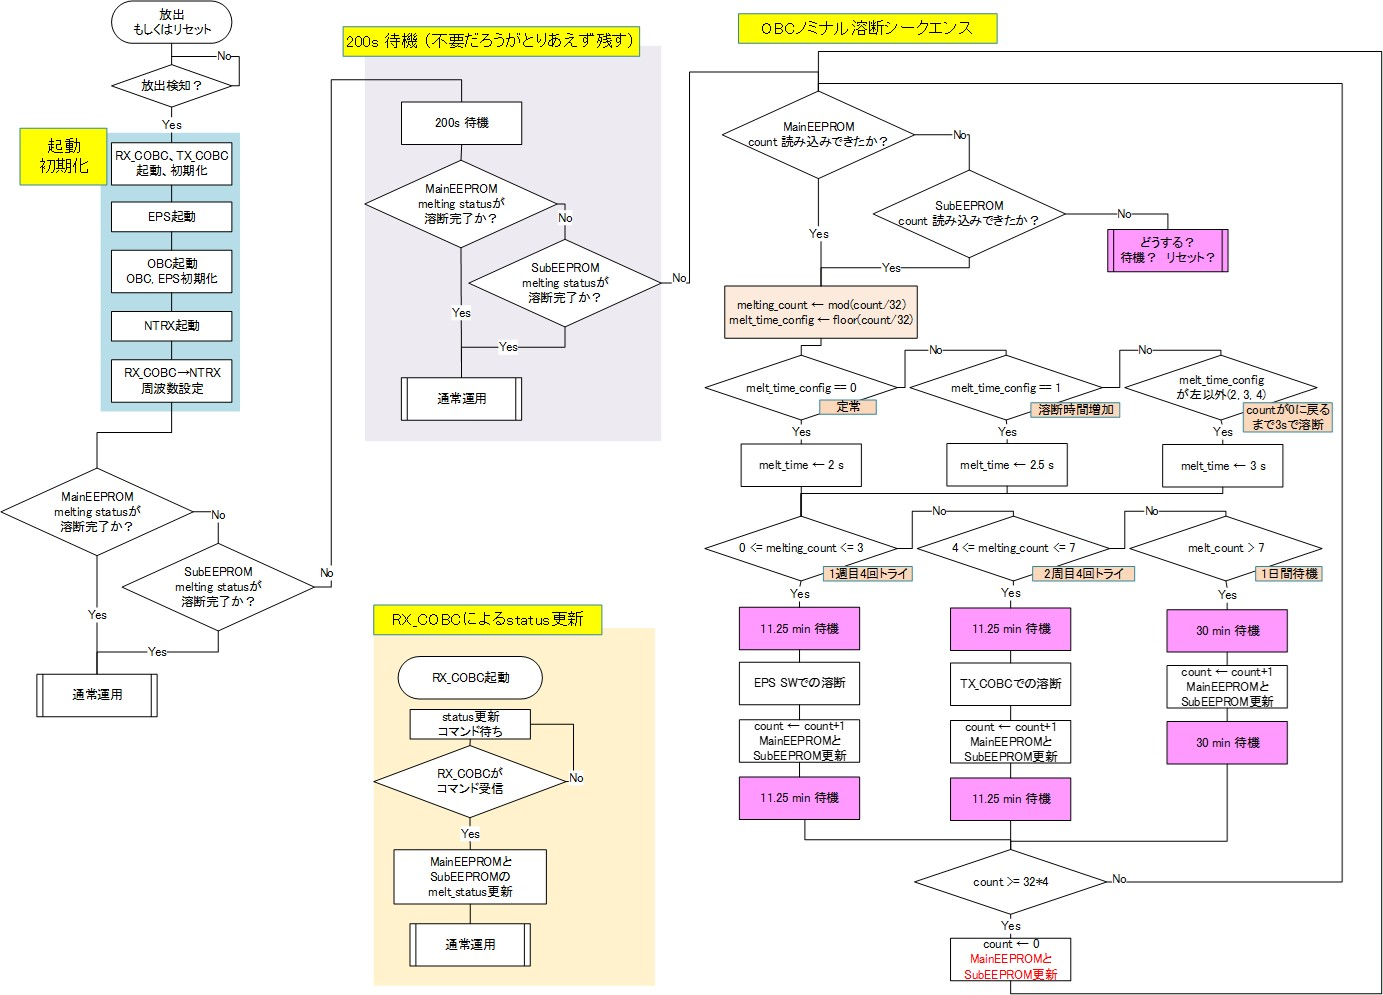
\includegraphics[scale=0.8,angle=90]{03/fig/3-4-Ini-1.pdf}
	\caption{OBCシート}
	\label{fig3-4-Ini-1}
\end{figure}

\subsubsection{OBC初期運用モードソフト詳細(小出)}
フローチャート的なものとセットで

\subsubsection{CIB初期運用モードソフト詳細(黒崎)}
フローチャート的なものとセットで

\subsubsection{初期運用 運用結果(余裕があれば黒崎.無理なら小出)}
CW HKデータで溶断済みを確認

\subsubsection{コメントや次回の改善点}
\hspace{2ex}
\textbf{OBC / CIB共通(黒崎・小出)}
\begin{itemize}
	\item 溶断済みフラグをCW HKデータのフリースペースの1byteに入れたのは神采配だったと思う.OrigamiSat-1の場合,アップリンクでEEPROMの指定アドレスを読んでダウンリンクする機能が使えなくなってしまっていたため,CW HKデータ以外に溶断済みを確認する術が無かった.
	\item OBCとCIBが同時に溶断を行ってしまった場合,バッテリーがどの程度減少するかの検証をできていなかった.
	\item OBCとCIBのどちらが,何回目の溶断で溶断を成功し,ダウンリンクを開始したかを分かるようにした方がいいのかもしれない.
\end{itemize}

\hspace{2ex}
\textbf{OBC(小出)}
\begin{itemize}
	\item aaaaaaaa
\end{itemize}

\hspace{2ex}
\textbf{CIB(黒崎)}
\begin{itemize}
	\item aaaaaaaa
\end{itemize}